\runningheader{SAT Mathematics}{Drill Set 7}{Page \thepage\ of \numpages}

\begingradingrange{sat-drill-07}
\subsection*{SAT Drill 7}


\question[1]
\begin{center}
\begin{tabular}{|l|l|l|}
\hline
\textbf{Value} & \textbf{Data set A frequency} & \textbf{Data set B frequency} \\
\hline
30 & 2 & 9 \\
\hline
34 & 4 & 7 \\
\hline
38 & 5 & 5 \\
\hline
42 & 7 & 4 \\
\hline
46 & 9 & 2 \\
\hline
\end{tabular}
\end{center}
Data set $A$ and data set $B$ each consist of 27 values. The table shows the frequencies of the values for each data set. Which of the following statements best compares the means of the two data sets?
\begin{choices}
  \choice The mean of data set $A$ is greater than the mean of data set $B$.
  \choice The mean of data set $A$ is less than the mean of data set $B$.
  \CorrectChoice The mean of data set $A$ is equal to the mean of data set $B$.
  \choice There is not enough information to compare the means of the data sets.
\end{choices}






















  

\question[1]
A data set of 27 different numbers has a mean of 33 and a median of 33. A new data set is created by adding 7 to each number in the original data set that is greater than the median and subtracting 7 from each number in the original data set that is less than the median. Which of the following measures does NOT have the same value in both the original and new data sets?
\begin{choices}
  \choice Median
  \choice Mean
  \choice Sum of the numbers
  \CorrectChoice Standard deviation
\end{choices}

\question[1]
What is the median of the data shown?\\
$$73,74,75,77,79,82,84,85,91$$
\begin{solution}
79
\end{solution}

\question[1]
\begin{center}
\begin{tabular}{|l|l|l|}
\hline
\multicolumn{3}{|c|}{International Tourist Arrivals, in millions} \\
\hline
\textbf{Country} & \textbf{2012} & \textbf{2013} \\
\hline
France & 83.0 & 84.7 \\
\hline
United States & 66.7 & 69.8 \\
\hline
Spain & 57.5 & 60.7 \\
\hline
China & 57.7 & 55.7 \\
\hline
Italy & 46.4 & 47.7 \\
\hline
Turkey & 35.7 & 37.8 \\
\hline
Germany & 30.4 & 31.5 \\
\hline
United Kingdom & 26.3 & 32.2 \\
\hline
Russia & 24.7 & 28.4 \\
\hline
\end{tabular}
\end{center}
The table above shows the number of international tourist arrivals, rounded to the nearest tenth of a million, to the top nine tourist destinations in both 2012 and 2013. Based on the information given in the table, how much greater, in millions, was the median number of international tourist arrivals to the top nine tourist destinations in 2013 than the median number in 2012, to the nearest tenth of a million?
\begin{solution}
1.3
\end{solution}


  











\question[1]
The dot plots represent the distributions of values in data sets $A$ and $B$.
\begin{center}
\begin{tabular}{cc}
Data Set A. & Data Set B. \\
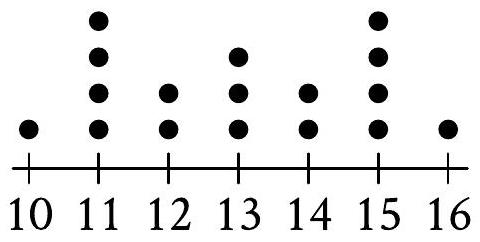
\includegraphics[width=0.23\textwidth]{images/2025_06_15_04f7426dc644de311e92g-15(1)} &
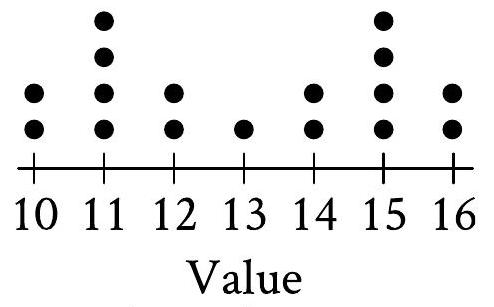
\includegraphics[width=0.23\textwidth]{images/2025_06_15_04f7426dc644de311e92g-15} \\
\end{tabular}
\end{center}
Which of the following statements must be true?
\begin{enumerate}[label=(\Roman*)]
  \item The median of data set $A$ is equal to the median of data set $B$.
  \item The standard deviation of data set $A$ is equal to the standard deviation of data set $B$.
\end{enumerate}
\begin{choices}
  \choice I only
  \choice II only
  \choice I and II
  \choice Neither I nor II
\end{choices}

  

\question[1]
\insertimage{0.40}{images/2025_06_15_04f7426dc644de311e92g-16}{reference attached}
Two data sets of 23 integers each are summarized in the histograms shown. For each of the histograms, the first interval represents the frequency of integers greater than or equal to 10, but less than 20. The second interval represents the frequency of integers greater than or equal to 20, but less than 30, and so on. What is the smallest possible difference between the mean of data set $A$ and the mean of data set $B$?
\begin{choices}
  \choice 0
  \choice 1
  \choice 10
  \choice 23
\end{choices}

\question[1]
What is the mean of the data shown?\\
$$2,9,14,23,32$$
\begin{choices}
  \choice 14
  \CorrectChoice 16
  \choice 17
  \choice 32
\end{choices}






















  

\question[1]
\begin{center}
\begin{tabular}{|c|c|}
\hline
Value & Frequency (probability) \\
\hline
1 & $a$ \\
\hline
2 & $2a$ \\
\hline
3 & $3a$ \\
\hline
4 & $2a$ \\
\hline
5 & $a$ \\
\hline
\end{tabular}
\end{center}
The frequency distribution above summarizes a set of data, where $a$ is a positive integer. How much greater is the mean of the set of data than the median?
\begin{choices}
  \CorrectChoice 0
  \choice 1
  \choice 2
  \choice 3
\end{choices}

\question[1]
Two different teams consisting of 10 members each ran in a race. Each member's completion time of the race was recorded. The mean of the completion times for each team was calculated and is shown below.\\
Team A: 3.41 minutes\\
Team B: 3.79 minutes\\
Which of the following MUST be true?
\begin{enumerate}[label=(\Roman*)]
  \item Every member of team $A$ completed the race in less time than any member of team $B$.
  \item The median time it took the members of team B to complete the race is greater than the median time it took the members of team A to complete the race.
  \item There is at least one member of team B who took more time to complete the race than some member of team A.
\end{enumerate}
\begin{choices}
  \CorrectChoice III only
  \choice I and III only
  \choice II and III only
  \choice I, II, and III
\end{choices}






























  

\question[1]
The mean score of 8 players in a basketball game was 14.5 points. If the highest individual score is removed, the mean score of the remaining 7 players becomes 12 points. What was the highest score?
\begin{choices}
  \choice 20
  \choice 24
  \CorrectChoice 32
  \choice 36
\end{choices}

\question[1]
\insertimage{0.40}{images/2025_06_15_c6d1fe032100fbb48447g-11}{reference attached}
Which of the following equations is the most appropriate linear model for the data shown in the scatterplot?
\begin{choices}
  \choice $y=-1.9x-10.1$
  \choice $y=-1.9x+10.1$
  \choice $y=1.9x-10.1$
  \choice $y=1.9x+10.1$
\end{choices}

  

\question[1]
A study was done to determine a new car's stopping distance when it was traveling at different speeds. The study was done on a dry road with good surface conditions. The results are shown below, along with the graph of a quadratic function that models the data.
\insertimage{0.40}{images/2025_06_15_c6d1fe032100fbb48447g-12}{reference attached}
According to the model, which of the following is the best estimate for the stopping distance, in feet, if the vehicle was traveling 55 miles per hour?
\begin{choices}
  \choice 25
  \choice 30
  \choice 210
  \choice 250
\end{choices}


  

\question[1]
The scatterplot shows the temperature $y$, in ${ }^{\circ} \mathrm{F}$, recorded by a meteorologist at various times $x$, in days since June 1.
\insertimage{0.40}{images/2025_06_15_c6d1fe032100fbb48447g-13}{reference attached}
During which of the following time periods did the greatest increase in recorded temperature take place?
\begin{choices}
  \choice From $x=6$ to $x=7$
  \choice From $x=5$ to $x=6$
  \choice From $x=2$ to $x=3$
  \choice From $x=1$ to $x=2$
\end{choices}





































  

\question[1]
\insertimage{0.40}{images/2025_06_15_c6d1fe032100fbb48447g-14}{reference attached}
Which of the following could be the equation for a line of best fit for the data shown in the scatterplot above?
\begin{choices}
  \choice $y=3x+0.8$
  \choice $y=0.8x+3$
  \choice $y=-0.8x+3$
  \choice $y=-3x+0.8$
\end{choices}

  

\question[1]
The scatterplot below shows the amount of electric energy generated, in millions of megawatt-hours, by nuclear sources over a 10-year period.
\insertimage{0.40}{images/2025_06_15_c6d1fe032100fbb48447g-15}{reference attached}
Of the following equations, which best models the data in the scatterplot?
\begin{choices}
  \choice $y=1.674x^{2}+19.76x-745.73$
  \choice $y=-1.674x^{2}-19.76x-745.73$
  \choice $y=1.674x^{2}+19.76x+745.73$
  \choice $y=-1.674x^{2}+19.76x+745.73$
\end{choices}

  

\question[1]
\insertimage{0.40}{images/2025_06_15_c6d1fe032100fbb48447g-16}{reference attached}
Each dot in the scatterplot above represents the temperature and the number of people who visited a beach in Lagos, Nigeria, on one of eleven different days. The line of best fit for the data is also shown. According to the line of best fit, what is the number of people, rounded to the nearest 10, predicted to visit this beach on a day with an average temperature of $32^{\circ} \mathrm{C}$?
\begin{choices}
  \choice 440
  \choice 460
  \choice 480
  \choice 500
\end{choices}


  

\question[1]
The line graph shows the estimated number of chipmunks in a state park on April 1 of each year from 1989 to 1999.
\insertimage{0.40}{images/2025_06_15_c6d1fe032100fbb48447g-17}{reference attached}
Based on the line graph, in which year was the estimated number of chipmunks in the state park the greatest?
\begin{choices}
  \choice 1989
  \choice 1994
  \choice 1995
  \choice 1998
\end{choices}

\question[1]
In which of the following tables is the relationship between the values of $x$ and their corresponding $y$-values nonlinear?
\begin{choices}
  \choice
  \begin{center}
  \begin{tabular}{|r|r|r|r|r|}
  \hline
  $x$ & 1 & 2 & 3 & 4 \\
  \hline
  $y$ & 8 & 11 & 14 & 17 \\
  \hline
  \end{tabular}
  \end{center}

  \choice
  \begin{center}
  \begin{tabular}{|l|l|l|r|r|}
  \hline
  $x$ & 1 & 2 & 3 & 4 \\
  \hline
  $y$ & 4 & 8 & 12 & 16 \\
  \hline
  \end{tabular}
  \end{center}

  \choice
  \begin{center}
  \begin{tabular}{|r|r|r|r|r|}
  \hline
  $x$ & 1 & 2 & 3 & 4 \\
  \hline
  $y$ & 8 & 13 & 18 & 23 \\
  \hline
  \end{tabular}
  \end{center}

  \CorrectChoice
  \begin{center}
  \begin{tabular}{|r|r|r|r|r|}
  \hline
  $x$ & 1 & 2 & 3 & 4 \\
  \hline
  $y$ & 6 & 12 & 24 & 48 \\
  \hline
  \end{tabular}
  \end{center}
\end{choices}


  



























\question[1]
\insertimage{0.40}{images/2025_06_15_c6d1fe032100fbb48447g-19}{reference attached}
The graph above shows the relationship between the speed of a particular car, in miles per hour, and its corresponding braking distance, in feet. Approximately how many feet greater will the car's braking distance be when the car is traveling at 50 miles per hour than when the car is traveling at 30 miles per hour?
\begin{choices}
  \choice 75
  \choice 125
  \choice 175
  \choice 250
\end{choices}

\question[1]
\insertimage{0.40}{images/2025_06_15_c6d1fe032100fbb48447g-20}{reference attached}
Which of the following could be an equation for a line of best fit for the data in the scatterplot?
\begin{choices}
  \choice $y=-x+6$
  \choice $y=-x-6$
  \choice $y=6x+1$
  \choice $y=6x-1$
\end{choices}

\question[1]
A wind turbine completes 900 revolutions in 50 minutes. At this rate, how many revolutions per minute does this turbine complete?
\begin{choices}
  \CorrectChoice 18
  \choice 850
  \choice 950
  \choice 1,400
\end{choices}

\question[1]
\begin{center}
\begin{tabular}{|c|c|}
\hline
$x$ & $y$ \\
\hline
1 & 4 \\
\hline
3 & 12 \\
\hline
5 & 20 \\
\hline
40 & $k$ \\
\hline
\end{tabular}
\end{center}
In the table above, the ratio of $y$ to $x$ for each ordered pair is constant. What is the value of $k$?
\begin{choices}
  \choice 28
  \choice 36
  \choice 80
  \CorrectChoice 160
\end{choices}












































\question[1]
\begin{center}
\begin{tabular}{|c|c|}
\hline
Species of tree & Growth factor \\
\hline
Red maple & 4.5 \\
\hline
River birch & 3.5 \\
\hline
Cottonwood & 2.0 \\
\hline
Black walnut & 4.5 \\
\hline
White birch & 5.0 \\
\hline
American elm & 4.0 \\
\hline
Pin oak & 3.0 \\
\hline
Shagbark hickory & 7.5 \\
\hline
\end{tabular}
\end{center}
One method of calculating the approximate age, in years, of a tree of a particular species is to multiply the diameter of the tree, in inches, by a constant called the growth factor for that species. The table above gives the growth factors for eight species of trees. If a white birch tree and a pin oak tree each now have a diameter of 1 foot, which of the following will be closest to the difference, in inches, of their diameters 10 years from now? (1 foot = 12 inches)
\begin{choices}
  \choice 1.0
  \choice 1.2
  \CorrectChoice 1.3
  \choice 1.4
\end{choices}

\question[1]
The ratio of $t$ to $u$ is 1 to 2, and $t=10$.\\
What is the value of $u$?
\begin{choices}
  \choice 2
  \choice 5
  \choice 10
  \CorrectChoice 20
\end{choices}

\question[1]
A special camera is used for underwater ocean research. When the camera is at a depth of 58 fathoms, what is the camera's depth in feet? (1 fathom = 6 feet)
\begin{solution}
348
\end{solution}

\question[1]
A sample of oak has a density of 807 kilograms per cubic meter. The sample is in the shape of a cube, where each edge has a length of 0.90 meters. To the nearest whole number, what is the mass, in kilograms, of this sample?
\begin{choices}
  \CorrectChoice 588
  \choice 726
  \choice 897
  \choice 1,107
\end{choices}

\question[1]
On April 18, 1775, Paul Revere set off on his midnight ride from Charlestown to Lexington. 
If he had ridden straight to Lexington without stopping, he would have traveled 11 miles 
in 26 minutes. In such a ride, what would the average speed of his horse have been, to 
the nearest tenth of a mile per \underbar{hour}?
\begin{solution}
25.4
\end{solution}

  

































\question[1]
How many yards are equivalent to 612 inches? (1 yard = 36 inches)
\begin{choices}
  \choice 0.059
  \CorrectChoice 17
  \choice 576
  \choice 22,032
\end{choices}

\question[1]
Rectangle $A$ has length 15 and width $w$. Rectangle $B$ has length 20 and the same length-to-width ratio as rectangle $A$. What is the width of rectangle $B$ in terms of $w$?
\begin{choices}
  \CorrectChoice $\frac{4}{3}w$
  \choice $w+5$
  \choice $\frac{3}{4}w$
  \choice $w-5$
\end{choices}

\question[1]
Shaquan has 7 red cards and 28 blue cards. What is the ratio of red cards to blue cards that Shaquan has?
\begin{choices}
  \CorrectChoice 1 to 4
  \choice 4 to 1
  \choice 1 to 7
  \choice 7 to 1
\end{choices}

\question[1]
Last year, Cedric had 35 plants in his garden. This year, the number of plants in Cedric's garden is $60\%$ greater than the number of plants in his garden last year. How many plants does Cedric have in his garden this year?
\begin{solution}
56
\end{solution}

\question[1]
What is $23\%$ of 100?
\begin{choices}
  \CorrectChoice 23
  \choice 46
  \choice 77
  \choice 123
\end{choices}

\question[1]
Which expression represents the result of increasing a positive quantity $w$ by $43\%$?
\begin{choices}
  \CorrectChoice $1.43w$
  \choice $0.57w$
  \choice $43w$
  \choice $0.43w$
\end{choices}

\question[1]
The population of City A increased by $7\%$ from 2015 to 2016. If the 2016 population is $k$ times the 2015 population, what is the value of $k$?
\begin{choices}
  \choice 0.07
  \choice 0.7
  \CorrectChoice 1.07
  \choice 1.7
\end{choices}














































\question[1]
What is $10\%$ of 470?
\begin{choices}
  \choice 37
  \CorrectChoice 47
  \choice 423
  \choice 460
\end{choices}

\question[1]
Which of the following represents the result of increasing the quantity $x$ by $9\%$, where $x>0$?
\begin{choices}
  \CorrectChoice $1.09x$
  \choice $0.09x$
  \choice $x+9$
  \choice $x+0.09$
\end{choices}

\question[1]
The number $k$ is $36\%$ greater than 50. If $k$ is the product of 50 and $r$, what is the value of $r$?
\begin{choices}
  \choice 36
  \choice 3.6
  \CorrectChoice 1.36
  \choice 0.36
\end{choices}

\question[1]
The number $a$ is $70\%$ less than the positive number $b$. The number $c$ is $80\%$ greater than $a$. The number $c$ is how many times $b$?
\begin{solution}
0.54
\end{solution}

\question[1]
210 is $p\%$ greater than 30. What is the value of $p$?
\begin{solution}
600
\end{solution}

\question[1]
The value of $z$ is 1.13 times 100. The value of $z$ is what percent greater than 100?
\begin{choices}
  \choice 11.3
  \CorrectChoice 13
  \choice 130
  \choice 213
\end{choices}

\question[1]
A city has 50 city council members. A reporter polled a random sample of 20 city council members and found that 6 of those polled supported a specific bill. Based on the sample, which of the following is the best estimate of the number of city council members in the city who support the bill?
\begin{choices}
  \choice 6
  \choice 9
  \CorrectChoice 15
  \choice 30
\end{choices}
























\question[1]
A study was done on the weights of different types of fish in a pond. A random sample of fish were caught and marked in order to ensure that none were weighed more than once. The sample contained 150 largemouth bass, of which $30\%$ weighed more than 2 pounds. Which of the following conclusions is best supported by the sample data?
\begin{choices}
  \choice The majority of all fish in the pond weigh less than 2 pounds.
  \choice The average weight of all fish in the pond is approximately 2 pounds.
  \choice Approximately $30\%$ of all fish in the pond weigh more than 2 pounds.
  \CorrectChoice Approximately $30\%$ of all largemouth bass in the pond weigh more than 2 pounds.
\end{choices}

\question[1]
A park ranger asked a random sample of visitors how far they hiked during their visit. Based on the responses, the estimated mean was found to be 4.5 miles, with an associated margin of error of 0.5 miles. Which of the following is the best conclusion from these data?
\begin{choices}
  \choice It is likely that all visitors hiked between 4 and 5 miles.
  \choice It is likely that most visitors hiked exactly 4.5 miles.
  \choice It is not possible that any visitor hiked less than 3 miles.
  \CorrectChoice It is plausible that the mean distance hiked for all visitors is between 4 and 5 miles.
\end{choices}

  

\question[1]
\begin{center}
\begin{tabular}{|c|c|c|c|}
\hline
Coat color & \multicolumn{3}{|c|}{Eye color} \\
\hline
 & Deep blue & Light brown & Total \\
\hline
Cream-tortoiseshell & 16 & 16 & 32 \\
\hline
Chocolate & 12 & 4 & 16 \\
\hline
Total & 28 & 20 & 48 \\
\hline
\end{tabular}
\end{center}
The data on the coat color and eye color for 48 Himalayan kittens available for adoption were collected and summarized in the table above. What fraction of the chocolate-colored kittens has deep blue eyes?
\begin{choices}
  \choice $\frac{12}{48}$
  \choice $\frac{12}{28}$
  \choice $\frac{16}{32}$
  \CorrectChoice $\frac{12}{16}$
\end{choices}

\question[1]
\begin{center}
\begin{tabular}{|l|c|c|c|c|c|}
\hline
High school & \multicolumn{5}{|c|}{Year} \\
\hline
 & 2008 & 2009 & 2010 & 2011 & 2012 \\
\hline
Foothill & 87 & 80 & 75 & 76 & 70 \\
\hline
Valley & 44 & 54 & 65 & 76 & 82 \\
\hline
Total & 131 & 134 & 140 & 152 & 152 \\
\hline
\end{tabular}
\end{center}
The table above shows the number of students from two different high schools who completed summer internships in each of five years. No student attended both schools. Of the students who completed a summer internship in 2010, which of the following represents the fraction of students who were from Valley High School?
\begin{choices}
  \choice $\frac{10}{140}$
  \CorrectChoice $\frac{65}{140}$
  \choice $\frac{75}{140}$
  \choice $\frac{65}{75}$
\end{choices}

  

































\end{enumerate}

\question[1]
\begin{center}
\begin{tabular}{|c|c|}
\hline
Voice type & Number of singers \\
\hline
Countertenor & 4 \\
\hline
Tenor & 6 \\
\hline
Baritone & 10 \\
\hline
Bass & 5 \\
\hline
\end{tabular}
\end{center}
A total of 25 men registered for singing lessons. The frequency table shows how many of these singers have certain voice types. If one of these singers is selected at random, what is the probability he is a baritone?
\begin{choices}
  \choice 0.10
  \CorrectChoice 0.40
  \choice 0.60
  \choice 0.67
\end{choices}

\question[1]
A survey taken by 1,000 students at a school asked whether they played school sports. The table below summarizes all 1,000 responses from the students surveyed.
\begin{center}
\begin{tabular}{|l|c|c|}
\hline
 & Males & Females \\
\hline
Play a school sport & 312 & 220 \\
\hline
Do not play a school sport & $?$ & 216 \\
\hline
\end{tabular}
\end{center}
How many of the males surveyed responded that they do not play a school sport?
\begin{choices}
  \choice 109
  \CorrectChoice 252
  \choice 468
  \choice 688
\end{choices}

\question[1]
\begin{center}
\begin{tabular}{|c|c|c|c|c|}
\hline
 & \multicolumn{4}{|c|}{Blood type} \\
\hline
Rhesus factor & A & B & AB & O \\
\hline
+ & 33 & 9 & 3 & 37 \\
\hline
- & 7 & 2 & 1 & $x$ \\
\hline
\end{tabular}
\end{center}
Human blood can be classified into four common blood types-A, B, AB, and O. It is also characterized by the presence $(+)$ or absence $(-)$ of the rhesus factor. The table above shows the distribution of blood type and rhesus factor for a group of people. If one of these people who is rhesus negative $(-)$ is chosen at random, the probability that the person has blood type $B$ is $\frac{1}{9}$. What is the value of $x$?
\begin{solution}
8
\end{solution}

\question[1]
A survey was conducted using a sample of history professors selected at random from the California State Universities. The professors surveyed were asked to name the publishers of their current texts. What is the largest population to which the results of the survey can be generalized?
\begin{choices}
  \choice All professors in the United States
  \choice All history professors in the United States
  \CorrectChoice All history professors at all California State Universities
  \choice All professors at all California State Universities
\end{choices}

\question[1]
The members of a city council wanted to assess the opinions of all city residents about converting an open field into a dog park. The council surveyed a sample of 500 city residents who own dogs. The survey showed that the majority of those sampled were in favor of the dog park. Which of the following is true about the city council's survey?
\begin{choices}
  \choice It shows that the majority of city residents are in favor of the dog park.
  \choice The survey sample should have included more residents who are dog owners.
  \choice The survey sample should have consisted entirely of residents who do not own dogs.
  \CorrectChoice The survey sample is biased because it is not representative of all city residents.
\end{choices}

